\documentclass[11pt,conference]{IEEEtran}
\usepackage[utf8]{inputenc}
\usepackage[english]{babel}
\usepackage{graphicx}
\graphicspath{ {images/} }

\begin{document}

\section{Approach}
Our original plan was to utilize ROS on Linux to interface with the Kinect, but we were unable to get the drivers to work with our model of Kinect and opted instead to use the Kinect SDK for Windows. After analyzing this technology for some time, we decided that the best approach to the problem was to break it down into three smaller subproblems: raw data acquisition, production of models for use with libSVM, and gesture matching. The first two deal with specifying the gestures that were ultimately used in the system, while the last actually recognized them. Each of these subproblems was dealt with by its own program, which we will detail here.
\subsection{Raw Data Acquisition}
The first program gathered joint data from the Kinect and placed it in a file. After initializing the Kinect and setting it up to capture skeleton data, the program entered into a data capture loop. Here, the program waits until it starts receiving meaningful data. Once it does, it outputs the data to a file and to the screen, waits for 200 milliseconds, and repeats the process until 25 frames of data have been captured. The file is formatted with each line containing the frame number, joint number, x coordinate of the joint, y coordinate, and z coordinate.

\begin{figure}[h]
\caption{A portion of the raw data file.}
\centering
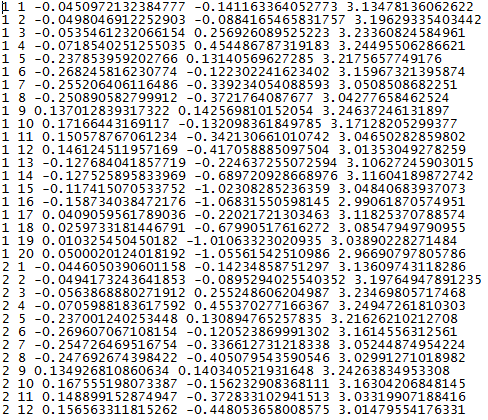
\includegraphics[width=\linewidth]{raw_data}
\end{figure}

Because all of our gestures are static, 25 frames seemed like a good amount of data to collect. It is small enough that the actor does not have to stand for too long, yet large enough to capture some good data. In retrospect, it may have helped to improve our accuracy if we had experimented with which number of frames gave us the best accuracy.

The Kinect does not always produce good data; on occasion, the skeleton will appear ``jittery." To help rectify this, we wait 200 milliseconds between frames. This reduces some of that jitter, which important for our training set in particular. It also allows the program operator to quickly browse over some of the incoming data to ensure that it appears to be meaningful.

\subsection{Production of Models For Use With LIBSVM}

\subsection{Gesture Matching}
\end{document}